\documentclass[12pt]{article}

\usepackage{afterpage}
\usepackage{amsmath}
\usepackage{amssymb}
\usepackage{times}
\usepackage[style=authoryear, natbib=true, backend=biber, doi=false,isbn=false,url=false]{biblatex}
\addbibresource{./fieldbib.bib}
\usepackage{cite}
\usepackage{natbib}
\usepackage{url}
\usepackage{float}
\usepackage[nottoc, notlof]{tocbibind}
\usepackage{graphicx}
\usepackage{ctable}
\usepackage{caption}
\usepackage{multirow}
\usepackage{threeparttable}
%\usepackage{subfigure}
\usepackage{amsthm}
\usepackage{fullpage}
\usepackage{enumerate}
\usepackage{setspace}
\usepackage{epigraph}
\usepackage{appendix}
\usepackage{etoolbox}
\usepackage{bm} %use \boldsymbol{} for greek bold
\usepackage{mathrsfs} %$\mathscr{L}$ or B for script letters
\apptocmd{\sloppy}{\hbadness 10000\relax}{}{}
\usepackage{chngcntr}
\usepackage{framed}
\usepackage{pdflscape}
\usepackage{longtable}
\usepackage{subcaption}
\usepackage{pdfpages}
\usepackage{arydshln} % for dashed hline: \hdashline
\usepackage{caption}
\usepackage{rotating}

\newcommand{\diff}{\mbox{Diff}}
\newcommand{\R}{\mathbb{R}}
\newcommand{\N}{\mathbb{N}}
\renewcommand{\P}{\mathcal{P}}
\newcommand{\e}{\varepsilon}
\newcommand{\av}{\mbox{Av}}
\renewcommand{\l}{\lim_{n\rightarrow\infty}}
\newcommand{\be}{\mathbf{e}}
\newcommand{\bA}{\mathbf{A}}
\newcommand{\bS}{\mathbf{\Sigma}}
\newcommand{\bI}{\mathbf{I}}
\newcommand{\bU}{\mathbf{U}}
\newcommand{\bone}{\mathbf{1}}
\newcommand{\bM}{\mathbf{M}}
\renewcommand{\wp}{\succeq}
\renewcommand{\sp}{\succ}
\newcommand{\wlp}{\preceq}
\newcommand{\slp}{\prec}
\newcommand{\ind}{\sim}
\newcommand{\B}{\mathscr{B}}
\renewcommand{\L}{\mathscr{L}}
\newcommand{\der}[2]{\ensuremath{\dfrac{\partial #1}{\partial 
#2}}}
\renewcommand{\a}[1]{\begin{align*}#1\end{align*}}
\newcommand{\anum}[1]{\begin{align}#1\end{align}}
\renewcommand{\citet}[1]{\citeauthor{#1} \citeyearpar{#1}}


%\bibpunct{(}{)}{;}{a}{,}{,}


\frenchspacing

%\doublespace

% \setcounter{secnumdepth}{0}

% \renewcommand*\thechapter{\Roman{chapter}}
% \renewcommand*\thepart{\Roman{part}}
% %\renewcommand*\thesection{\arabic{section}.}
% \renewcommand*\thesubsection{\Alph{subsection}.}
% \renewcommand*\thesubsubsection{\roman{subsubsection}}
% \renewcommand*\theparagraph{\thesubsubsection}
% \renewcommand*\thesubparagraph{\thesubsubsection}
% %\renewcommand*\subsection{\thesection.}
% %\renewcommand*\subsubsection{\thesubsection.}
% %\renewcommand*\paragraph{\thesubsubsection.}
% %\renewcommand*\subparagraph{\theparagraph.}

% \setcounter{tocdepth}{1}
% 


% \usepackage{titlesec}
% \titleformat{\chapter}[display]{\normalfont\centering\bfseries}{\MakeUppercase{\chaptertitlename}~\MakeUppercase{\thechapter}}{12pt}{\MakeUppercase}
% \titleformat{\section}[display]{\normalfont\centering\bfseries}{\thesection}{}{}
% \titleformat{\subsection}[display]{\normalfont\bfseries}{\thesubsection}{}{}

% \usepackage[parfill]{parskip}

\newcommand{\ght}{\citep{greenstone2014} }
\newcommand{\gha}{\citet{greenstone2014} }
\newcommand{\did}{differences-in-differences }

\begin{document}

\maketitle



\section*{Abstract}
\singlespacing
Differences-in-differences estimators can be biased in the presence of treatment externalities. In this paper I develop a spatial model that accounts for these externalities, and estimate the model using data on Indian river pollution. I show that failing to account for treatment externalities can substantially bias estimates toward zero.
The Indian government built 107 sewage treatment plants in 1995 as part of the National River Conservation Plan (NRCP). The general consensus in the literature and among the Indian population is that the NRCP has been largely ineffective. Using data from the Central Pollution Control Board's river monitoring network, I find significant reductions in measured pollution levels in the areas downstream of sewage treatment facilities when compared to untreated areas. 

\pagebreak 

\doublespacing

\section{Introduction} \label{sec:intro}

\defcitealias{css}{CSS, 2015}

India's waterways are heavily utilized and dangerously polluted. As of 2007, there were just 234 sewage treatment plants in all of India \citep{cpcb2008}. In contrast, the United States has 14,780 sewage treatment plants \citepalias{css}, despite having a quarter of the population. In 2011, India's Ministry of Environment and Forests estimated that existing sewage treatment plants have the capacity to treat less than one third of all municipal sewage. In most cases, untreated sewage is discharged directly into a river or other body of water. 

The dangerous pollution levels in India's waterways constitute a public health disaster. Millions of Indian citizens rely on water from polluted rivers for drinking, bathing, and cleaning. In addition, many rivers are considered holy in the Hindu faith and are believed to have purifying effects. Each year, millions of pilgrims ceremonially drink from, and bathe in, polluted rivers. 

India's government is aware of the problem and has taken steps to address it. Beginning in 1985 under the Ganga Action Plan, 865 billion USD has been allocated for reducing river pollution across the country. However, it is widely held that the various cleanup schemes implemented by the government have been a failure \citep{hindu}. In a 2009 interview, Minister of State for Environment and Forests Jairam Ramesh stated that widescale changes to the government's approach were needed or else resources would ``continue to be wasted'' \citep{indiatoday}.

Despite this popular perception, there has been no systematic study of the effectiveness of any specific policy intervention at the national level. This paper addresses this gap by estimating the effect of new sewage treatment plant (STP) construction on pollution levels in India's rivers. In 1995, over one hundred new STPs were built at various locations around India as part of the National River Conservation Plan (NRCP). I estimate the effect of these STPs on pollution levels using data from the Central Pollution Control Board's network of river-monitoring stations. In a preview of the main results, I find that STP construction has been associated with a small but significant decrease in pollution levels, but the effects diminish in the long run.

The differences-in-differences estimator is commonly used when estimating the average treatment effect of a policy change. However, spillovers (or externalities) occur when treatment affects observations that are not directly targeted by the policy. These spillovers can contaminate the control group in a \did setting, therefore leading to biased estimates of the true treatment effect. In this paper, I address this issue in the context of river pollution abatement in India. I find that failing to account for treatment spillovers can substantially bias \did estimates in this setting. 

The findings presented here are directly relevant to Indian policymakers. Despite the perception of waste and ineffectiveness, I find that STP construction can potentially reduce pollution to levels that are considered safe for bathing and recreational activity. 

The baseline result is shown using a simple \did approach implemented with OLS, as is standard in the development literature \citep{greenstone2015}. However, the existence of treatment externalities may confound identification. Aquatic pollutants mix non-uniformly across space; pollution generated at one point along a river will be present downstream, but natural remediation processes will work to reduce pollution levels as the downstream distance increases. The existence of a sewage treatment plant reduces pollution at the closest downstream monitoring station, but also reduces pollution at all subsequent downstream monitoring stations. This constitutes a treatment externality. Failing to account for treatment externalities can bias \did estimators \citep{miguel2004}. 

Error processes may persist downstream as well. Any shock that directly affects pollution levels measured at an upstream monitoring station will potentially affect all downstream monitoring stations. Failing to account for this downstream error process can result in distorted inferences. I therefore develop a spatial econometric model which allows both treatment effects and errors to persist downstream \citep{anselin1988, lesage2009}. In a novel contribution to the spatial literature, I specify an exponential spatial lag to capture the downstream effects of pollution. Under this parameterization, the spatial model is equivalent to nonlinear least squares with exponential decay of the dependent variable. This model has wide-ranging applications in environmental and development settings, in situations where treatment effects diminish exponentially over distance or time. 

In the next section, I review related research in the environmental and development literature. The data are discribed in Section \ref{sec:data}. Section \ref{sec:ols} presents OLS estimation results. As outlined above, the covariance matrix of simple OLS models is likely misspecified if pollution persists downstream. The novel spatial model that accounts for this error process is presented and estimated in \mbox{Section \ref{sec:spat}}. I discuss the policy significance of the results in \mbox{Section \ref{sec:disc}} before concluding with Section \ref{sec:conclusion}.

\section{Related Literature} \label{sec:lit}

\citet{greenstone2015} highlight the importance of identifying (a) the mechanisms that contribute to high pollution levels in the developing world, and (b) which policy measures are effective at reducing exposure to pollution. They emphasize that pollution abatement depends not only on the marginal willingness to pay for abatement for those who are affected by pollution, but also on the institutional environment that builds and maintains the necessary abatement infrastructure. Large utility gains may go unrealized due to weak institutions; resources may be misallocated to the extent that abatement measures are never undertaken.

The ability of the Indian government to implement efficient water pollution abatement measures is analyzed in \citet{greenstone2014}. They utilize a \did approach to estimate the average effect on pollution levels when certain cities are designated as ``problem areas'' by the Indian government, relative to cities that receive no such designation. They find that the problem-area designation is not associated with any decrease in pollution levels, a result they attribute to the weak institutional environment in India. The \citeauthor{greenstone2014} result serves as the starting point for this paper. Here, I focus on a specific policy interve the construction of new STPs---which allows for a more precise identification of the institutional shortcomings. In particular, I find that STPs are initially effective at reducing pollution levels, but these effects are short-lived, likely due to the depreciation of physical and human capital.

In a similar study, \citet{lipscomb2015} use data from a Brazilian water-pollution monitoring network to estimate downstream pollution spillovers. They leverage variation in shifting county-border location between upstream-downstream station pairs (as a result of administrative redistricting) to find that pollution generation increases as borders downstream of monitoring stations move upstream; decentralized regulation and abatement authorities do not internalize the downstream effects of pollution and abatement. Each station-pair is treated as a unique observation in the data, and \citeauthor{lipscomb2015} apply OLS with standard heteroscedastic-robust standard errors. As I show in Section \ref{sec:spat}, this assumes that the errors are unrelated across station pairs, an assumption that is unlikely to hold along river systems. 

In contrast to \citeauthor{lipscomb2015}, I estimate the effects of a specific policy intervention (i.e. the construction of new sewage treatment plants). However, most of the existing literature on abatement focuses on air pollution rather than water pollution. For example, \citet{fowlie2012} analyze the effects of cap-and-trade schemes on pollution levels compared to the effects of command-and-control regulation. They exploit spatial variation in the regulatory environment to identify a significant decrease in pollution levels associated with the cap-and-trade policy. 

Using similar methodology, \citet{auffhammer2011} estimate the effects of gasoline regulation on air pollution. Identification is based on spatial variation in gasoline content laws across US states, aimed at reducing ozone created from emissions of volatile organic compound emissions. The heterogeneity of implementation across states allows them to identify which type of abatement measure is more effective. They find that measures aimed at the specific volatile organic compounds (those that are more likely to create ozone) are more effective than general quotas on emissions, because general quotas allow polluters to substitute toward other ozone-creating processes. 

The effects of heterogeneous abatement compliance identified in these previous studies are particularly acute in developing countries such as India. The estimation results in this paper suggest considerable heterogeneity across time in abatement effectiveness. In Section \ref{sec:disc}, I present evidence that a lack of operations oversight, as well as capital depreciation, are likely to blame, echoing the types of findings in the existing environmental literature. 

The importance of using quasi-experimental settings when analyzing abatement technologies is highlighted by \citet{dominici2014}. Identification based solely on spatial variation in a policy intervention is generally not sufficient to ensure unbiased estimates of a causal effect, because policies may be non-randomly implemented. In the present context, the locations of new sewage treatment facilities are likely to be non-random, but the downstream pollution effects are unlikely to suffer from the same problem. For example, the set of municipalities that construct new STPs will likely share unobserved characteristics that impact pollution levels. However, the pollution-generating processes downstream of these cities is plausibly random. If municipalities that discharge large amounts of raw sewage into a river are targeted, other downstream municipalities will derive benefit from the construction of an upstream STP, regardless of the level of sewage generation and existing abatement technology present at those downstream locations. As long as the unobserved characteristics common to locations with new STPs are orthogonal to the downstream location of each monitoring station, \citeauthor{dominici2014}'s exogeneity condition is likely satisfied.

If downstream monitoring stations on the same river are designated as ``controls'', the downstream effects of sewage treatment introduce spillovers into a \did estimation environment. In a very different context, \citet{miguel2004} estimate the effects of deworming medication on school-children in the presence of analogous spillovers. Children at schools that are randomly selected for treatment influence the health of other children in the same neighborhood---siblings and friends attending untreated schools in the same areas benefit from lower hookworm and roundworm infection rates among their peers. The authors control for this by including the total number of children who live within a certain distance of the treated students and the number of treated children within that same distance. This specification accounts for potential bias in point estimates due to treatment spillovers, but the estimated parameter variance-covariance matrix does not account for the same spatial dependence. For instance, an untreated child with a natural, unobserved immunity to hookworm infections will spread benefits to other untreated children, who have one less peer that may infect them. But this ``error'' is not captured in the estimation of the variance-covariance matrix.

The potential for bias when estimating covariance matrices is particularly problematic in an environmental setting. Both pollution generation and abatement have the potential to influence multiple locations (or individuals) simultaneously. Spatial econometric techniques can explicitly account for for this type of simultaneity, but they remain underutilized in both the environmental and development economics literature.

\section{Data} \label{sec:data}

India's Central Pollution Control Board (under the umbrella of the Ministry of Environment and Forests) maintains a network of 447 river-monitoring stations throughout India. Water samples are taken at specific time intervals (monthly or quarterly), and then sent to regional laboratories for analysis. Data on various pollutants measured at each station were compiled by \gha. Their sample covers the period from 1986 to 2004. 

These data also contain information about the geospatial location of each monitoring station. The geospatial information consists of a low-resolution coordinate (accurate to one minute of latitude and longitude---69 miles at the equator) and a brief physical description of the site (for example, the name of the bridge or public beach where the water samples are taken). I used this information in conjunction with Google Maps and OpenStreetMap to pinpoint the exact location of each pollution monitoring station.\footnote{Some monitoring stations could not be pinpointed using this method. In this case, the river location nearest to the centroid of the coordinate range was chosen. This strategy was implemented for fewer than 5\% of all monitoring stations in the data.} I then used the coordinates from these locations to calculate the great-circle distance between stations. Each monitoring station was then plotted using OpenStreetMap, allowing the exact upstream/downstream relationship between stations to be recorded. 

The 477 monitoring stations in India are located along 60 separate river systems (see Table \ref{tab:descstats}). Each river system therefore has an average of $7.45$ stations. For 28 of these river systems, there is only one monitoring station, while the largest river system (the Ganga) has 109 stations. 

\begin{table}[t!]
  \centering
  \caption{Descriptive Statisics}
  \label{tab:descstats}
  \begin{tabular}{ccccc}
    \hline
    Variable & Mean & St. Dev. & Min & Max \\
    \hline
    Log of Fecal Coliforms & 5.665 & 2.918 & 0.000 & 14.560 \\
    Distance to nearest upstream station\textsuperscript{\textdagger} & 52.410 & 61.178 & 0.278 & 385.700 \\
    Stations per river system & 7.450 & 17.476 & 1 & 109 \\
\hline 
\multicolumn{5}{p{.9\textwidth}}{\footnotesize{ \textdagger Measured in kilometers. Upstream distance calculated only for stations with upstream neighbors. Of the 447 monitoring stations, 148 have no associated upstream station.}}
\end{tabular}
\end{table}

Not all monitoring stations are active during every year of the sample period (Figure \ref{fig:year_counts}). New stations are continually added to the network, while some are removed. The overall trend is toward more monitoring stations, however. There were 114 active stations in 1986, but 398 by 2004. As a result, the upstream/downstream relationship between monitoring stations is not constant. Distance to the closest upstream station can decrease as new stations are added, or it can increase if the closest upstream station is not operational or reporting data in that time period.

\begin{figure}[t!] \centering 
	\includegraphics[scale=.65]{year_counts.pdf}
	\caption{Number of Monitoring Stations by Year}
	\label{fig:year_counts}
\end{figure}


\begin{figure}[t!]
  \centering
  \includegraphics[scale=.9]{hist}
  \caption{Distribution of Downstream Distances Between Monitoring Stations}
  \label{fig:dist}
\end{figure}
Figure \ref{fig:dist} shows the distribution of distances, across the 398 monitoring stations, and each of the station's closest downstream neighboring station (excluding those with no downstream neighbors). Roughly 62\% of all monitoring stations have another station within 50 kilometers downstream. Any pollution or abatement  process with even a modest downstream persistence is therefore likely to have its effects be detected at multiple downstream stations in the sample, potentially biasing a \did estimator. 

The water samples at each monitoring station are tested for a variety of pollutants and pollution indicators. The indicator utilized in this paper is the count of fecal coliforms (fcoli) in the water. The advantages of this indicator are threefold. First, fcoli is one of the most commonly monitored water pollution indicators in the environmental science literature. Concentrations of fcoli are well understood to be closely correlated with the overall health of a water body. Second, fcoli is the most commonly reported pollution indicator in the sample. Lastly, fcoli levels provide a direct measurement of the amount of untreated sewage in the water.

Fecal coliforms are a class of coliform bacteria that grow exclusively in the digestive tracts of mammals, feeding on digested food.\footnote{Most forms of fecal coliforms are not harmful to humans, with a few notable exceptions. For example, \textit{escherichia coli} (E. coli) is a form fecal coliform and can cause fatal illness.} Sewage treatment eliminates the food source, so properly treated wastewater therefore has very low levels of fcoli. The levels of fecal coliforms remaining in the water after treatment are thus the primary indicator for the effectiveness of sewage treatment. 

The counts of fcoli are generally reported in natural logs, a convention I follow in this paper. In the laboratory, water samples are added to an fcoli growth medium and left to incubate for a fixed period, after which the number of colonies can readily be counted. The colony growth over the incubation period is exponential, so taking the natural log allows for more robust comparisons of the actual number of coliforms present in the water source. 

\begin{figure}[t]
  \centering
  \includegraphics[scale=.85]{kde1.pdf}
  \caption{Sample Kernel Density Estimate of Fecal Coliforms}
  \label{fig:kde}
\end{figure}

\defcitealias{epa}{EPA 2012}

Figure \ref{fig:kde} shows the distribution of fcoli in the sample, across the panel of data consisting of all measurements at all stations. The dashed, vertical line represents the United States Environmental Protection Agency's ``statistical threshold value'' (STV) for fcoli levels in recreational water (similar regulatory criteria for India, if they have actually been established, are not publicly available). At this cutoff, recreational users of the water are likely to fall ill due to fcoli contamination at an estimated rate of 32/1000 \citepalias{epa}. Above this level, the EPA deems a body of water to be unsafe for recreational activity.

Nearly half (49\%) of all fcoli measurements in the Indian sample are above the EPA's STV. Simply bathing in an Indian river carries a substantial risk of contracting a waterborne illness. Given that millions of Indian citizens also rely on river water for cooking, cleaning, and drinking, the fcoli levels in India's rivers represent a significant public health crisis. 

One of the primary objectives of the National River Conservation Plan was the construction of new sewage treatment facilities. In 1995, 107 treatment plants were built along India's rivers \citep{nrcd2013}. The location of each of these STPs was obtained from the Ministry of Environment and Forests and verified based on satellite photos from Google Earth. The locations of each monitoring station and each STP are shown in Figure \ref{fig:map}. 

\begin{figure}[!t]
  \centering
  \includegraphics[scale=1]{map_small.pdf}
  \caption{107 Sewage Treatment Facilities and 447 Monitoring Stations}
  \label{fig:map}
\end{figure}

The effect of STP construction on pollution levels is empirically identified based on the siting of the STPs. Fcoli counts at monitoring stations upstream of STPs are compared to counts at monitoring stations downstream, before and after construction of the STP is completed. The wide geographic dispersion of both monitoring stations and STPs helps to ensure that the estimates are reasonably representative for India.


\section{OLS Results} \label{sec:ols}

Least-squares estimation can recover unbiased estimates of treatment externalities if the spatial structure is properly specified. Robust parameter standard-error estimation, however, requires the error variance-covariance matrix be properly specified as well. In this section, I ignore the potential problems with estimating the error covariance structure and consider a simple, parsimonious model. Despite the potential for biased parameter standard errors, this estimation strategy is common in the literature. The results reported in this section are best viewed as a baseline. In Section \ref{sec:spat} we will see that the OLS estimates are quantitatively similar to those obtained from the more robust spatial model, though the OLS estimates of the long-run effect (five or more years after treatment) are likely biased toward zero.

\subsection{Na\"{i}ve Difference-in-Differences Estimation}

Following the approach used in many development and environmental settings \citep{greenstone2015}, I specify a simple difference-in-differences model as a baseline. This approach measures the treatment effect on the treated stations relative to the never-treated stations. This model is written as:
\anum{
	P_{it} &= \beta_1 T_{it} + \beta_2 (t\cdot D_{i}) + \beta_3 (t \cdot T_{it}) + \tau_t + \psi_i + \e_{it} \label{eq:baseline} \\
	\e_{it} &\sim N(0, \sigma^2_i), \nonumber
}
where $P_{it}$ is the measured pollution level at station $i$ at time $t$, $D_{i}$ is a dummy variable indicating whether station $i$ is treated at any time in the sample, and $T_{it}$ is a dummy variable equal to 1 if station $i$ is treated in time $t$. The parameters $\tau_t$ and $\psi_i$ are station- and time-specific fixed effects which control for any unobserved sources of heterogeneity that are constant across time and stations. The term $\beta_2 (t\cdot D_{i})$ allows for pollution levels at treated stations to evolve on a differential trend from that of the untreated stations, while $\beta_3 (t \cdot T_{it})$ allows for a structural break in that trend at the treatment date. 

Each station is considered treated if it is immediately downstream of an STP, and untreated otherwise. This ``na\"{i}ve'' specification captures the first-order effect of sewage treatment on the downstream station relative to all other stations, including those downstream. That is, the indirect effects of treatment on other stations downstream of an STP are assumed to be zero. Later, however, this assumption will be relaxed. 


\begin{sidewaystable}[ph!] \centering \footnotesize
  \caption{Na\"{i}ve Differences-in-Differences Estimates} 
  \label{tab:1} 
\begin{tabular}{@{\extracolsep{5pt}}lccccccc} 
\\[-1.8ex]\hline 
\hline \\[-1.8ex] 
 & \multicolumn{7}{c}{\textit{Dependent variable:}} \\ 
\cline{2-8} 
\\[-1.8ex] & \multicolumn{7}{c}{Log of Fecal Coliforms} \\ 
\\[-1.8ex] & (1) & (2) & (3) & (4) & (5) & (6) & (7)\\ 
\hline \\[-1.8ex] 
 Treatment Effect ($\beta_1$) & $-$0.388$^{***}$ & $-$1.266$^{***}$ & $-$1.165$^{***}$ & $-$0.816$^{***}$ & $-$0.873$^{***}$ & $-$0.759$^{***}$ & $-$0.773$^{***}$ \\ 
  & (0.066) & (0.113) & (0.115) & (0.076) & (0.117) & (0.118) & (0.118) \\ 
  & & & & & & & \\ 
Pre-treatment Trend ($\beta_2$) &  & 0.008$^{***}$ & 0.004$^{**}$ & 0.032 &  & $-$0.002 & 0.004$^{**}$ \\ 
  &  & (0.001) & (0.002) & (0.033) & & (0.001) & (0.002) \\ 
  & & & & & & & \\ 
Post-treatment Trend ($\beta_3$) &  &  & 0.006$^{***}$ & 0.013$^{***}$ & &  & $-$0.013$^{***}$ \\ 
  &  &  & (0.002) & (0.002) & &  & (0.003) \\ 
  & & & & & & \\ 
 Post 5 Year Effect ($\beta^L_1$) & & &  &  & 0.995$^{***}$ & 1.085$^{***}$ & 1.499$^{***}$ \\ 
  &  &  & & & (0.073) & (0.105) & (0.129) \\ 
  & & & & & & & \\ 
Long-run Effect ($\beta_1 + \beta_1^L$) & & &  &  & 0.122$^*$ & 0.326$^*$ & 0.7256$^{***}$ \\ 
 & &  &  &  & (0.073) & (0.188) & (0.206) \\ 
\hline \\[-1.8ex] 
Station-specific time trends & No & No & No & Yes & No & No & No \\
R$^{2}$ & 0.620 & 0.621 & 0.621 & 0.631 & 0.622 & 0.622 & 0.622 \\ 
Adjusted R$^{2}$ & 0.613 & 0.614 & 0.614 & 0.624 & 0.615 & 0.615 & 0.615 \\  
\hline
\hline \\[-1.8ex] 
\multicolumn{8}{p{.9\textwidth}}{\footnotesize{\textit{Note:} $^{*}$p$<$0.1; $^{**}$p$<$0.05; $^{***}$p$<$0.01. Heteroskedastic-robust standard errors in parentheses. All regressions have 38,625 observations and contain time and station fixed-effects. Estimation results for equation \eqref{eq:baseline} are in columns 1-5. Equation \eqref{eq:post5} is reported in column 6.} }
\end{tabular} 
\end{sidewaystable} 



Table \ref{tab:1} shows the results of the na\"{i}ve \did model (equation \eqref{eq:baseline}). \mbox{Column 1} reports the simple treatment effect in levels with no allowance for differential trends between the treated and untreated groups ($\beta_2 = \beta_3 = 0$). The estimated treatment effect is small but statistically significant, indicating that the average pollution levels at the stations immediately downstream of an STP are lower, on average, throughout the post-treatment period relative to the pre-treatment period.

Columns 2 and 3 of Table \ref{tab:1} report the estimates for the model with a pre-treatment trend (column 2) and with both pre- and post- treatment trends (column 3). Over the entire sample period, stations immediately downstream of an STP have a positive and significant trend in their pollution levels relative to other stations ($\beta_2$, the coefficient on $t\cdot D_i$). This result can be explained by noting that the placement of STPs is nonrandom---it is likely that areas with increasing sewage generation were prioritized for intervention by policymakers. 

Specifying linear trends for the treated stations results in a much larger (in magnitude) estimated initial treatment effect---that is, the treatment effect in the first year following treatment. Furthermore, the slope of the post-treatment trend line ($\beta_2 + \beta_3$) is positive and steeper than the pre-treatment trend ($\beta_3 > 0$). Taken as a whole, the parameter estimates in columns 2 and 3 of Table \ref{tab:1} indicate that there is estimated time-heterogeneity in the treatment effect. Large, initial reductions in pollution are offset over time by an increase in the pollution trend of treated stations. 

The time-heterogeneity of the treatment effect can be analyzed by interacting the treatment variable with a full set of year dummies:
\anum{
	P_{it} &= \sum_{\tau} \beta_\tau T_{i\tau} + \delta_t + \psi_i + \e_{it}\label{eq:hettime} \\
	\e_{it} &\sim N(0, \sigma^2_i), \nonumber
}
where $T_{i\tau}$ is a dummy equal to one if station $i$ is treated in year $\tau$. The sequence $\{\hat{\beta}_\tau\}$ nonparametrically describes the time trend in treated stations relative to untreated stations. These coefficients can be interpreted as treatment-specific year fixed effects. 

Figure \ref{fig:1} plots the estimated $\hat{\beta}_\tau$'s along with their 95\% confidence intervals. Due to the linear dependence in equation \eqref{eq:hettime} (one dummy variable for each year in the sample), the year 1994 (the year before the STPs are built) is specified as the base year. Each $\hat{\beta}_\tau$ therefore measures the average level of pollution relative to the level measured in 1994. The results are striking---stations immediately downstream of sewage treatment facilities show a large, immediate decrease in their measured pollution levels. But the effect is short-lived: pollution levels begin to rise after three years, and are statistically insignificantly different from the pre-treatment levels just six years after the STPs are built. The slight upward trend in pre-treatment means reported in Table \ref{tab:1} can also be observed, although the coefficients on the indicators for each of the years immediately preceding treatment are statistically indistinguishable from one another. 

\begin{figure}[t] \centering 
	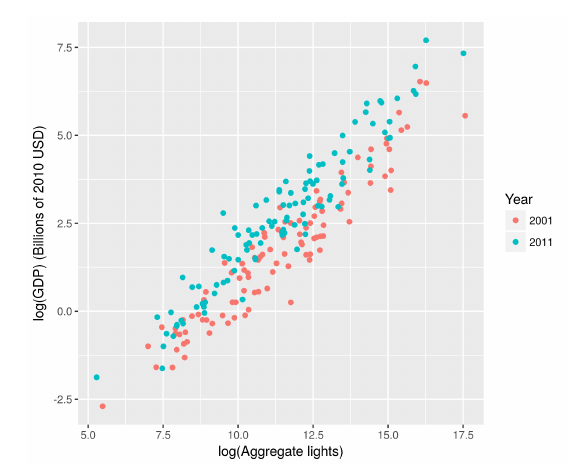
\includegraphics[scale=.9]{fig1}
	\caption{Treatment Effect by Year Relative to 1994}
	\label{fig:1}
\end{figure}

The results presented in Figure \ref{fig:1} motivate the estimation of a specification that distinguishes between short-run and long-run treatment effects:
\begin{align}
  	P_{it} &= \beta_1 T_{it} + \beta_1^L T_{it}^{L}+ \beta_2 (t\cdot D_{i}) + \beta_3 (t\cdot T_{it}) + \tau_t + \psi_i + \e_{it} \label{eq:post5}
\end{align}
The new variable $T_{it}^{L}$ is an indicator equal to one if station $i$ is treated and $t$ is at least six years after the initial treatment date. 

The estimation results are reported in Columns 5, 6, and 7 of Table \ref{tab:1}. The estimated coefficient on $T^L_{it}$ is positive and significant in all specifications. In fact, the estimated rise in pollution levels at treated stations five years after treatment is large enough to overcome the initial reduction. The estimated level effect of treatment after five years is given by $\beta_1 + \beta_1^L$, which is estimated to be positive and significantly different from zero (at the 10\% level) in all specifications. 

These results offer one possible explanation for why the effects of the NRCP have not been previously observed. Studies comparing pollution levels a few years after the construction of an STP might find little to no effect, despite the substantial decrease immediately following treatment. The potential reasons for this mean-reverting behavior of measured pollution levels will be discussed in Section \ref{sec:disc}.

\subsection{Treatment Externalities} \label{sec:ols_poly}

The identifying assumption underlying the na\"{i}ve specifications in equations \eqref{eq:baseline} and \eqref{eq:hettime} is that the construction of an STP impacts pollution levels only at the nearest station immediately downstream. As discussed in Section \ref{sec:intro}, this assumption is unlikely to hold. In particular, other stations farther downstream from the ``treated'' stations may also see a reduction in pollution levels, though to a smaller extent than stations closer to the STPs (if there is some natural remediation or dilution process that occurs naturally). Estimated treatment effects are likely biased in the presence of these treatment externalities as downstream monitors are considered as ``controls,'' but these controls are contaminated by the upstream treatment.

To account for this bias I consider the alternative specification:
\begin{subequations}
\anum{
	P_{it} &=  \sum_{s} \Phi_n(d_{si})\widetilde{T}_{s i t} + \tau_t + \psi_i + \e_{it} \label{eq:treatext} \\
	\Phi_n(d_{si}) &= \beta_0 + \beta_1 d_{si} + \beta_2 d_{si}^2 + \dots + \beta_n d_{si}^n \label{eq:poly} \\
	\e_{it} &\sim N(0, \sigma^2_i).\nonumber
}
\end{subequations}

The variable $d_{si}$ measures the downstream distance of monitoring station $i$ from STP $s$. $\Phi_n(d)$ is an n\textsuperscript{th}-order polynomial of downstream distance (in kilometers), which allows for treatment effects to vary over distance. $\widetilde{T}_{sit}$ is new treatment indicator equal to one if station $i$ is anywhere downstream of STP $s$ in time $t$. For each monitoring station $i$, the distance polynomial is summed over all upstream STPs. Each station can therefore potentially be treated by multiple STPs simultaneously. 

The above specification considers all stations downstream of an STP as treated. The intensity of treatment thus varies across the number of upstream STPs and the downstream distance of each monitoring station from each STP (connected by a river system). In contrast to the model in equation \eqref{eq:baseline}, this specification explicitly accounts for treatment externalities. Identification is based on the number of upstream STPs and the variation in distance between each station and each upstream STPs. 

\begin{table}[t!] \centering 
  \caption{Downstream Abatement Effects }
  \label{tab:downstream} 
\begin{tabular}{@{\extracolsep{5pt}}llccccc} 
\\[-1.8ex]\hline 
\hline \\[-1.8ex] 
 & & \multicolumn{5}{c}{\textit{Dependent variable:}} \\ 
\cline{3-7} 
\\[-1.8ex] & & \multicolumn{5}{c}{Log of Fecal Coliforms} \\ 
\\[-1.8ex] 
\small{Coefficient} & \small{Variable} & (1) & (2) & (3) & (4) & (5)\\ 
\hline \\[-1.8ex] 
 $\beta_0$ & $\widetilde{T}_{sit}$ & $-$0.227$^{***}$ & $-$0.454$^{***}$ & $-$0.553$^{***}$ & $-$0.338$^{***}$ & $-$0.418$^{***}$ \\ 
&  & (0.020) & (0.026) & (0.046) & (0.055) & (0.024) \\ 
 & & & & & & \\ 
 $\beta_1$ & $d/ 1000$ & 0.315$^{***}$ & 1.422$^{***}$ & 2.376$^{***}$ & $-$0.981 & 0 \\ 
&  & (0.027) & (0.082) & (0.375) & (0.615) &  \\ 
&  & & & & & \\ 
 $\beta_2$ & $(d/ 1000)^2$ &  & $-$0.808$^{***}$ & $-$2.607$^{***}$ & 9.296$^{***}$ & 6.412$^{***}$ \\ 
&  &  & (0.056) & (0.690) & (1.804) & (0.485) \\ 
 & & & & & & \\ 
 $\beta_3$ & $(d/ 1000)^3$ &  &  & 0.892$^{***}$ & $-$13.553$^{***}$ & $-$10.505$^{***}$ \\ 
&  &  &  & (0.340) & (1.991) & (0.935) \\ 
  & & & & & & \\ 
 $\beta_4$ & $(d/ 1000)^4$ & &  &  & 5.536$^{***}$ & 4.484$^{***}$ \\ 
&  &  &  &  & (0.736) & (0.448) \\ 
 & & & & & & \\ 
\hline \\[-1.8ex] 
\multicolumn{2}{l}{Polynomial Order}  & 1 & 2 & 3 & 4 & 4 \\ 
\multicolumn{2}{l}{AIC}  & 156214.1 & 156009.2 & 156002.5 & 155949.5 & 155950.6 \\ 
\multicolumn{2}{l}{BIC}  & 162010.3 & 161814 & 161815.8 & 161771.4 & 161763.9 \\ 
\multicolumn{2}{l}{R$^{2}$}  & 0.621 & 0.623 & 0.623 & 0.624 & 0.624 \\ 
\multicolumn{2}{l}{Adjusted R$^{2}$} & 0.614 & 0.616 & 0.616 & 0.617 & 0.617 \\ 
\hline 
\hline \\[-1.8ex] 
\multicolumn{7}{p{.95\textwidth}}{\footnotesize{\textit{Note: } $^{*}$p$<$0.1; $^{**}$p$<$0.05; $^{***}$p$<$0.01.  Heteroskedastic-robust standard errors in parentheses. Coefficient estimates for distance measures ($d_{si}$) are scaled by a factor of $1,000$km. All specifications have 38,625 observations and include time and monitoring-station fixed-effects. Estimation results correspond to equation \eqref{eq:treatext}}} \\ 
\end{tabular} 
\end{table} 

Estimation results are given in Table \ref{tab:downstream}. Column 1 shows the results of a first-order polynomial specification, where the downstream effects are assumed to be linear in distance. Both estimated polynomial coefficients have the expected sign---initial decreases in pollution immediately downstream of an STP ($d=0$) dissipate as distance increases.

It is unlikely that downstream pollution effects are linear in distance. Column 2 corresponds to a polynomial order of two ($\Phi_2(\cdot)$), the most parsimonious specification that allows for nonlinearities. All of the coefficients are statistically significant at the 0.01 level. The ``treatment effect'' estimate, $\hat{\beta}_0$, is the predicted change in pollution levels at the location where an STP is constructed (downstream distance is 0km). The point estimate of $-0.454$ is more than 10\% larger in magnitude than the simple \did estimate reported in Table \ref{tab:1}. This indicates that failing to account for treatment externalities can substantially bias point-estimates toward zero. 

The polynomial specification also allows for the downstream effects to be analyzed. Note that 
\anum{ \der{\widehat{P}_{s,t}^2}{d_{i,s,t} \partial \widetilde{T}} = \Phi_n'(d_{i,s,t}). \label{eq:deriv} }
The treatment effects diminish as downstream distance increases only if $\Phi_n'(d_{sit}) > 0$. As expected, this condition is satisfied with the second-order polynomial $\Phi_2(\cdot)$ in column 2---treatment effects appear to be larger when a station is nearer to an STP. 

The third-order polynomial specification in column 3 shows an even larger estimated treatment effect than the second-order specification. In contrast, the fourth-order results in column 4 differ substantially. Of particular interest is the non-monotonic downstream treatment effect. ($\Phi'(d_{sit})<0$ when $d < 60.5$). This specification predicts an initial \textit{increase} in the magnitude of the estimated treatment effect over the first 60.5 kilometers downstream. This result is driven entirely by $\widehat{\beta}_1$, the coefficient on $d_{sit}$. Note that estimated sign is negative, indicating that the minimum of the polynomial function occurs when $d$ is positive. It is unlikely that the true treatment effect reaches its maximum 60.5 km downstream of an STP rather than immediately downstream. This observed behavior in the fourth-order polynomial is probably due to overfitting. 

The treatment effects estimated here reflect the average impact of abatement. There is some heterogeneity across rivers and STP locations---rate of flow and river volume are unfortunately not observed in the data. This heterogeneity may impact estimated downstream effects. Swift-moving water may ``carry'' the treatment effect downstream more effectively than stagnant rivers. The high-order polynomial specifications may capture some of this heterogeneous effect, thus giving rise to unexpected (but statistically insignificant) non-monotonicity.

One way to address this non-monotonicity is simply to drop the first-order variable $d_{sit}$ from the regression ($\beta_1 = 0)$, since the estimated coefficient for this variable is not significantly different from zero anyway. Results of this estimation are reported in column 5 of \mbox{Table \ref{tab:1}}. The results are qualitatively similar to the other specifications, and all covariates are significant at the 1\% level. Furthermore, the BIC prefers the specification without the $d_{sit}$ term (column 5) to the specification where it is included (column 4). The AIC, which is less sensitive to additional parameters, shows only a marginal preference toward the more inclusive model. A monotonic downstream effect can therefore be estimated with little, if any, loss in model validity. 

The statistical significance of the downstream effect at any arbitrary distance $d$ can be ascertained by performing a simple F-test on the linear hypothesis
\begin{align}
  H_0: \Phi_n(d) = 0.
\end{align} 
Figure \ref{fig:downstream} shows the estimated downstream effects of abatement for each of the specifications in Table \ref{tab:1}, along with 95\% confidence intervals. The estimates are similar for all of the non-linear specifications (polynomials of order 2 or above). In particular, the downstream effects do not become statistically indistinguishable from zero until 300 or 400 kilometers downstream, indicating a high degree of downstream persistence in the data. The non-monotonic downstream behavior of the 4th-order polynomial specification is also visible, but the initially wide confidence interval indicates uncertainty about the true shape of the downstream effect over the first 100 kilometers. This initial uncertainty is substantially reduced when the parameter $\beta_1$ is set equal to zero, as in the last panel.

\begin{figure}[t!] \centering 
	\includegraphics[scale=.65]{downstream_11.pdf}
	\caption{Treatment Effect by Downstream Distance}
	\label{fig:downstream}
        \caption*{\footnotesize \textit{Note:} Shaded regions represent 95\% confidence intervals.}
\end{figure}

\section{Spatial Model} \label{sec:spat}

The primary shortcoming of the OLS-based approach is its inability to capture the complexity of the error process. Throughout the previous section, it was assumed that errors were independent across monitoring stations, which is unlikely to be the case. This study is the first to find an abatement effect at the national level for STPs in India, so it is imperative to model the errors properly to ensure that the inference is not merely an artifact of a misspecified error structure. 

Shocks to local pollution levels that are observed at one station are expected to be observed (to some extent) at all other downstream stations as well. Thus the error processes at stations along the same river are likely correlated. Moreover, the extent of this correlation should be smaller for stations separated by larger distances than for stations that are near to each other. This suggests that the commonly used cluster-robust standard errors are unlikely to be adequate, since within-cluster error covariances are not homogeneous for any level of clustering. For instance, error clustering at the river level assumes that monitoring stations located hundreds of kilometers apart along the same river will have the same error correlation as stations separated by just a few kilometers. Similarly, errors clustered at the individual station level assume that errors are independent across stations, even those stations located within the same metropolitan area.

In this section, I assume that the process that describes the downstream treatment effect is identical to the process that describes the downstream error process. This assumption says that the amount of pollution that flows downstream from a particular location is the same regardless of the pollution source. Permanent  changes in estimated pollution, such as the changes that would be observed after the construction of a new STP, impact downstream stations in an identical manner as transient changes, such as a holiday that decreases industrial production. In other words, the local effects of changes in the upstream pollution generation process are the same regardless of the source of the pollution. This type of spatial relationship can be fully described by a ``spatial autoregressive model'' \citep{anselin1988, lesage2009}.

To illustrate the spatial process, consider two monitoring stations, labeled $A$ and $B$, located on unconnected bodies of water. Each station has pollution observations in time period $t=1,2$, and an STP is constructed immediately upstream of $A$ at $t=2$ (while station $B$ remains untreated). The pollution at each monitoring station can be described by
\anum{
	P_{A,t} &= \beta T_{A,t} + \tau_t + \psi_A + \e_{A,t},~~~ \e_{A,t} \sim N(0, \sigma^2_A) \\
	P_{B,t} &= \tau_t + \psi_B + \e_{B,t},~~~ \e_{B,t} \sim N(0, \sigma^2_B)	
}
Now suppose that a river (or canal) is ``created'' between $A$ and $B$ such that the two monitoring stations are connected by a waterway, so $A$ is now $d$ kilometers upstream of $B$. The pollution that is measured at $A$ will also be present at some level at station $B$ (downstream of $A$). The amount of $P_{A,t}$ that is present at $B$ is $f(d)P_{A,t}$, where $f:\R_+ \rightarrow [0,1]$ measures the proportion of pollution that persists $d$ kilometers downstream. Then we have
\anum{
	P_{Bt} &= f(d)P_{At} + \tau_t + \psi_B + \e_{Bt}.
}
Note that even though $B$ is untreated, the decrease in pollution at station $A$ will affect $P_{Bt}$ through the term $f(d)P_{At}$. 

The system can then be described in matrix form as
\anum{
	\left[ \begin{matrix} P_{A1} \\ P_{A2} \\ P_{B1} \\ P_{B2} \end{matrix} \right]
	= 
	\left[\begin{matrix} 
		0 & 0 & 0 & 0 \\
		0 & 0 & 0 & 0 \\
		f(d) & 0 & 0 & 0 \\
		0 & f(d) & 0 & 0 		
	\end{matrix}\right]
	\left[ \begin{matrix} P_{A1} \\ P_{A2} \\ P_{B1} \\ P_{B2} \end{matrix} \right]
	+ \beta \left[ \begin{matrix} 0 \\ 1 \\ 0 \\ 0 \end{matrix} \right]
	+ \left[ \begin{matrix} \tau_1 \\ \tau_2 \\ \tau_1 \\ \tau_2 \end{matrix} \right]
	+ \left[ \begin{matrix} \psi_A \\ \psi_A \\ \psi_B \\ \psi_B \end{matrix} \right]
	+ \left[ \begin{matrix} \e_{A1} \\ \e_{A2} \\ \e_{B1} \\ \e_{B2} \end{matrix} \right] 
}
This equation can be written more succinctly as:
\anum{
	P = WP + \beta T + \tau + \psi + \e. \label{eq:spat}
}
The matrix $W$ is known in the spatial econometrics literature as a ``spatial weight matrix.'' It captures the upstream/downstream relationship between monitoring stations and allows for measured pollution at upstream stations to affect measured pollution at downstream stations. 

Pollution shocks which occur at station $A$ persist downstream and are observed at station $B$ as well, propagating through the matrix $W$. This specification allows average pollution levels (through the idiosyncratic fixed effects), as well as any pollution shocks to persist downstream in a similar fashion. Accounting for the error process in this way allows for more-robust inferences concerning the parameter $\beta$ in equation \ref{eq:spat}, where $\hat{\beta}$ is the average treatment effect estimate.

Estimation of \eqref{eq:spat} requires a specific functional form for $f$. One possibility is to use the polynomial specification utilized in Section \ref{sec:ols_poly}. However, the inability of the polynomial specification to ensure a monotonic treatment effect over distance is a shortcoming of that specification. In addition, the local nature of polynomial approximations to nonlinear functions means that the error in the predicted downstream effect is likely to increase as downstream distance increases. All the polynomial orders estimated in Section \ref{sec:ols_poly} became \textit{positive} at large distances, a result that is unlikely to be consistent with the underlying data generating process. 

To preclude these non-monotonic effects, I adopt an exponential form for the pollution process:
\anum{
	f(d) = e^{-\rho d}
}
In this specification, downstream pollution (and abatement effects) are assumed to decay exponentially as distance increases. In addition to solving the non-monotonicity and positive treatment effects problems that plague the polynomial model, the exponential pollution process is more parsimonious, requiring just a single additional parameter, namely the exponential rate of decay $\rho$. This parameter measures the average rate at which pollution decays as it flows downstream. Estimates of $\rho$ that are large in magnitude indicate that pollution decays rapidly downstream, implying also that pollution (and treatment) spillovers have little effect on downstream pollution. 

The full spatial model can be expressed as 
\begin{subequations}
\anum{
	P &= W(\rho)P + \beta \widehat{T} + \tau + \psi + \e \label{eq:spat1}\\
	\e &= M(\lambda) \xi \\
	\xi &\sim N(0, \sigma^2 I \omega) \nonumber \label{eq:spat3}
}
\end{subequations}
The spatial weight matrix $W(\rho)$ captures the distance between adjacent monitoring stations:
\anum{
	W(\rho)_{i,j} = \begin{cases} e^{-\rho d_{ij}}, &\text{ if $i$ immediately downstream of $j$ in time $t$} \\ 0, &\text{ otherwise} \end{cases}
}
The treatment vector $\widehat{T}$ is constructed similarly to equation \eqref{eq:baseline}, but each treated station is weighted by the distance between that station and its nearest upstream STP:
\anum{
	\widehat{T} = \begin{cases} e^{-\rho d_{s i}} &\text{ if station $s$ immediately downstream of STP $i$}, \\ 0 &\text{ otherwise} \end{cases} 
}

The vector $\omega$ weights the variance $\sigma^2$ for each station, which accounts for station-level heteroskedasticity. This vector is premultiplied by the additional spatial weight matrix $M(\lambda)$, which captures the correlation between stations located within a certain radius of each other in the geospatial dimension:
\anum{
	M(\lambda)_{i,j} = \begin{cases} e^{-\lambda d_{ij}}, &\text{ if $d_{ij} < \overline{d}$} \\ 0, &\text{ otherwise} \end{cases}
}
These additional spatial weights describe shocks that affect pollution levels at multiple stations which are not (necessarily) located along the same river system. For instance, regional weather patterns (such as rainfall) may impact pollution levels at multiple stations across rivers. The maximum distance parameter $\overline{d}$ gives $M(\lambda)$ some zero entries, which increases computational efficiency. In all specifications, $\overline{d}$ is set to 500 kilometers.\footnote{The results are not sensitive to the choice of $\overline{d}$. The estimated values of $\lambda$ in various specifications suggest that the halflife of nearby pollution shocks is less than one kilometer. The percentage of the shock that persists to the 500km boundary is machine zero.}

Solving for $P$ in equation \eqref{eq:spat1} yields
\anum{
	P &= \beta (I - W(\rho))^{-1} 	\widehat{T} + \widetilde{\tau} + \widetilde{\psi} + (I - W(\rho))^{-1}  M(\lambda) \xi \label{eq:solved}
}
Expressing the equation as in \eqref{eq:solved} highlights the downstream effects of treatment and the error process. The matrix $(I - W(\rho))^{-1}$ can be expressed as the infinite sum
\anum{
	(I - W(\rho))^{-1} = I + W(\rho) + W(\rho)^2 + \dots 
}
By construction, each nonzero entry of the matrix $W(\rho)$ is an exponential function of the distance between stations $i$ and $j$, with elements of this matrix given by $w(\rho)_{ij} = e^{-\rho d_{ij}}$. Entries are nonzero if and only if $i$ is immediately upstream of $j$; $W(\rho)$ captures the first-order relationship between stations. Therefore, the elements of the matrix $W(\rho)^k$ capture the (exponentiated) distance relationship between stations that are separated by $k$ stations along a river system. For instance, $w(\rho)_{ij}^{[2]}$ (the $ij$ element of matrix $W(\rho)^2$) is nonzero if $i$ and $j$ are separated by one station. 

To see this, suppose the intermediate station (between $i$ and $j$) is indexed by $h$. Then $w(\rho)_{ih} = e^{-\rho d_{ih}}$ and $w(\rho)_{hj} = e^{-\rho d_{hj}}$. Then, by pre-multiplying $W(\rho)$ by itself, the $ij$\textsuperscript{th} element of the squared matrix $W(\rho)^2$ is
\anum{
  w(\rho)_{ij}^{[2]} &= e^{-\rho d_{ih}}e^{-\rho d_{hj}} \\
  &= e^{-\rho (d_{ih} + d_{hj})} \\
  &= e^{-\rho d_{ij}}
}

Rivers are unidirectional; pollution that flows from station $i$ to $j$ must flow through the intermediate station $h$ as well. The river distance that the pollution travels is therefore the sum the intermediate distances. The novel approach introduced here specifies an exponential function of distance in the weight matrix, which captures this result in an intuitive way.

The infinite sum $(I - W(\rho))^{-1}$ then captures the exponential of the distance between each station and all upstream stations.\footnote{There are a finite number of stations along each river in the data. Therefore the matrix $W(\rho)^k$ contains only zeros when $k$ is large, and the sum is finite.} By interacting this matrix with the treatment variable $\widehat{T}$, the spatial lag model collapses to the the treatment externality model in \eqref{eq:treatext}, but with an exponential treatment variable:
\anum{
P_{it} &= \sum_{s} \beta \widehat{T}_{sit}e^{-\rho d_{i,s}} +  \tau_t + \psi_i + \e_{it} + \sum_{\text{j upstream of i}} \e_{jt} e^{-\rho d_{i,j}} \label{eq:spatspill}
}
Note the similarities between equation \eqref{eq:spatspill} and the OLS model of Section \ref{sec:ols} (equation \eqref{eq:treatext}). The only difference in the non-stochastic portions of these equations is that the polynomial function of distance in equation \eqref{eq:treatext} is replaced with an exponential function in equation \eqref{eq:spatspill}. 

In contrast to the OLS model of equation \eqref{eq:treatext}, the upstream error terms are included in the spatial model. The externality matrix $(I - W(\rho))^{-1}$ interacts with the disturbance term, allowing errors to persist downstream in a similar manner to the treatment externalities. The heteroskedastic-robust errors estimated in Section \ref{sec:ols} are unlikely to be accurate in the presence of externalities. In contrast to a simple clustered-error approach, the externality matrix in equation \eqref{eq:spat3} allows errors to decay exponentially, rather than specifying common covariances within arbitrarily designated clusters. 

\subsection{Estimating the Spatial Model}

The likelihood function for the spatial model in \eqref{eq:spat1}-\eqref{eq:spat3} and sufficient conditions for the existence of a maximum are given in \citet{anselin1988}. Although it can be shown that these conditions are met, the time and station fixed effects and the heterogeneous error weights give rise to a 1,124-dimensional parameter space. Estimating the maximum and Fisher information is computationally infeasible at present.  

I instead estimate the spatial model using Bayesian techniques, as outlined by \citet{lesage2009}. A Bayesian posterior distribution is simply the weighted average of prior beliefs and the likelihood function. Rather than relying on the curvature (the Hessian matrix) at the maximum of the likelihood function to conduct hypothesis tests, Bayesian techniques can be used to estimate the entire posterior distribution, which can be used to express confidence in particular parameter values. Whenever feasible, I employ uniform priors.\footnote{I use the term ``uniform'' to refer to non-informative priors, where equal prior probability is assigned to each draw.} Furthermore, Bayesian posterior distributions converge to the likelihood function as the sample size approaches infinity. The posterior distributions reported here are therefore close approximations to the traditional likelihood function associated with the model. 

In general, the posterior distribution cannot be found analytically. Fortunately, various methods exist that allow for samples to be drawn from the posterior. A large number of samples can then be combined in a Monte-Carlo simulation of the true posterior distribution. Most sampling methods require samples to follow sequentially from the previous sample, forming ``chains'' of samples. Draws are not independent of each other, and it therefore takes a long time to cover a majority of the posterior distribution. For this reason, it is common practice to include a ``burn-in period'' wherein chains are initiated and samples are created, but the early samples are then discarded before the Monte-Carlo integration takes place. This burn-in allows the sampler to move away from the initial value and toward the mass of the posterior, thereby minimizing the impact of the initial draws (which are chosen by the researcher). Convergence of the chains can be analyzed by initializing various chains with heterogeneous starting values, then comparing the chains to see if they converge to similar regions of the parameter space.

In this paper I utilize the No-U-Turn sampler of \citet{homan2014}. This sampler is characterized by minimal path dependence and rapid convergence to the posterior distribution \citep{neal2011}. Given the large parameter space and the complexity of the likelihood function, these features are necessary to ensure convergence. 

The parameter space is minimized by drawing each unique element of $\omega$ from an inverse gamma distribution, where the shape and scale hyperparameters of the inverse gamma are drawn from a uniform distribution before each iteration. Uniform priors are assigned for each of the fixed effects. The exponential decay terms $\rho$ and $\lambda$ are assigned exponential priors with an inverse-scale parameter of 1. These priors account for the fact that the likelihood function is approximately uniform for large values of $\rho$ and $\lambda$, which correspond to very small externalities.\footnote{Without specifying these priors, the sampling algorithm tends to get ``stuck'' in regions with high draws of the exponential parameters, which delays convergence of the posterior draws. }


The No-U-Turn sampler is implemented using the Stan language \citep{carpenter2015}. Column 1 of Table \ref{tab:spat} shows the summary statistics for the posterior distributions. The estimated treatment effect is similar in magnitude to the effect estimated in the previous section. Following the sampler's burn-in period, none of the samples were greater than 0 (in fact, none of the samples were larger than $-0.2$). Recalling that the posterior distribution is quantitatively similar to the likelihood function, it can be concluded with near absolute certainty that the true treatment effect on measured downstream water pollution is negative and nonzero. 

\subsection{Estimation Results}

\begin{table}[t!] \centering
	\caption{Bayesian Spatial Estimation Results} 
	\label{tab:spat} 
	\begin{tabular}{@{\extracolsep{5pt}}lcc} 
		\\[-1.8ex]\hline 
		\hline \\[-1.8ex] 
		& \multicolumn{2}{c}{\textit{Dependent variable:}} \\ 
		\cline{2-3} 
		\\[-1.8ex] & \multicolumn{2}{c}{Log of Fecal Coliforms} \\ 
		\\[-1.8ex] & (1) & (2)\\ 
		\hline \\[-1.8ex] 
		Treatment ($\beta$)& $-$0.351 & $-$0.474 \\ 
		& [$-$0.406, $-$0.298] & [$-$0.402, $-$0.551] \\ 
		& & \\ 
		Post 5-Year Effect ($\beta^L$)&  & 0.216 \\ 
		&  & [0.144, 0.296] \\ 
		& & \\ 
                Long-Run Effect ($\beta + \beta^L$)& & $-$0.258 \\
                & & [$-$0.191, $-$0.324] \\
                & & \\
		Downstream Effect ($\rho$) & 0.006 & 0.009 \\ 
		& [0.005, 0.007] & [0.006 0.013] \\ 
		& & \\ 
		Regional Effect ($\lambda$) & 1.850 & 1.105 \\
		& [1.097, 2.913] & [0.531, 2.022] \\ 
		& & \\ 
		\hline \\[-1.8ex]
		Downstream Half-Life & 115.1 & 75.8 \\
		& [93.6, 140.5] & [54.8, 103.7] \\ 
		& & \\ 
		\hline 
		\hline \\[-1.8ex] 
		\multicolumn{3}{p{.75\textwidth}}{\footnotesize{\textit{Note:} Point estimates are posterior means. 95\% posterior likelihood in brackets. All specification include station and time fixed-effects and have 38,625 observations. Column 1 corresponds to equation \eqref{eq:solved} and column 2 corresponds to equation \eqref{eq:spathettime}.}}
	\end{tabular} 
\end{table}

Posterior summary statistics for the two spatial parameters are also reported in Table \ref{tab:spat}. The posterior mean for the estimate of $\lambda$ is substantially higher than that of $\rho$, indicating that regional pollution spillovers (between rivers) are relatively unimportant when compared to downstream pollution spillovers (within rivers). The mean draw from the posterior of $\lambda$ corresponds to a pollution-distance ``half-life'' of $0.387$ kilometers, which implies that 95\% of pollution disappears across rivers within 1.6 kilometers. Regional shocks appear to influence only those stations that are very near each other geospatially, such as stations located along different rivers within the same city. 

In contrast, the within-river spillover effect is much more substantial. The posterior mean of $\rho$ is $0.006$, which corresponds to a downstream half-life of $115.1$ kilometers. Upstream pollution, and therefore upstream pollution abatement, persists downstream for hundreds of kilometers. Ninety-five percent of pollution measured at some location on a river dissipates after an estimated 499.3 kilometers downstream.

\begin{figure}[t] \centering 
	\includegraphics[scale=.9]{spatial1}
	\caption{Bayesian Posterior Distributions}
	\label{fig:spatial1}
\end{figure}
	
Figure \ref{fig:spatial1} plots a kernel density estimate of the
posterior distributions presented in Table \ref{tab:spat}. Of
particular interest is the noticeable right-skewness in the posterior
distribution for $\lambda$. The sampler periodically selects large values which correspond to very small regional effects. If assigned a uniform prior, the sampler has difficulty converging to a distribution with a finite mean---the sampler converges only by discounting the large draws of $\lambda$. This suggests that regional spillovers are even less significant than the point estimates suggest. Shock processes that have a common effect on stations across rivers appear to have little influence on pollution levels beyond a few kilometers.


\begin{figure}[t] \centering 
	\includegraphics[scale=.9]{trace}
	\caption{Bayesian Posterior Draws}
	\label{fig:trace}
\end{figure}

Figure \ref{fig:trace} shows the trace plot for the posterior draws. Each line represents the posterior draws associated with one of the 32 chains that were initiated (burn-in period included). The rapid convergence of the No-U-Turn sampler is apparent; for all initial values, the sampler converges to the posterior distribution after only 50 draws. Initial values of the treatment effect $\beta$ range from $-1.937$ to $2.003$, and all chains quickly converge to the posterior centered on $-0.351$. Initial values of $\rho$ are between $0.150$ and $5.992$, with all chains converging to the posterior mean of $0.006$ within $50$ draws. The estimates are therefore robust to a wide range of arbitrary initial values, and the rapid convergence of all chains suggests that the true posterior distribution is being sampled.

The results in Section \ref{sec:ols} suggested that the treatment effect is heterogeneous across time. This heterogeneity is investigated in the spatial setting by estimating the equation
\anum{
  P & = W(\rho)P + \beta \widehat{T} + \beta^L \widehat{T}^L + \tau + \psi + \e, \label{eq:spathettime}
}
which is the spatial analogue of equation \eqref{eq:post5}. $\widehat{T}$ is again the treatment variable, weighted by the downstream distance from the STP. $\widehat{T}^L$ is similarly defined, but is equal to zero for the first five years after the date when the sewage treatment plant is built, as in equation \eqref{eq:post5}. $\beta$ is therefore the treatment effect for just the first five years after treatment, while $\beta + \beta^L$ is the long-run effect. 

Similar to the results in Section \ref{sec:ols}, the treatment effect is found to be larger in the first five years after treatment (column 2 of Table \ref{tab:spat}). The short-run treatment effect of $0.474$ is cut in half after five years, indicating that the sewage treatment plants, on average, lose about half of their effectiveness after five years of operation. 

In contrast to Section \ref{sec:ols}, the long-run treatment effect ($\beta + \beta^L$) remains negative and significant. The spatial dependencies in the data appear to bias the long-run OLS estimates toward zero. The richer model that accounts for the spatial lag shows a significant effect on pollution levels downstream of sewage treatment plants even after the initial five-year period. Despite evidence of substantially reduced effectiveness over time, the sewage treatment plants still appear to have a significant long-run beneficial impact on pollution levels. 

\begin{figure}[t] \centering 
	\includegraphics[scale=.9]{spatial2}
	\caption{Bayesian Posterior Distributions \\ Heterogeneous Treatment}
	\label{fig:spatial2}
\end{figure}

\subsection{Joint Posterior Distributions}

The estimates of the spillover parameter $\rho$ in column 2 of Table \ref{tab:spat} remains similar to that of column 1. While the mean of the posterior shifts substantially, this is mostly due to an increase in the right-hand tail of the posterior distribution (Figure \ref{fig:spatial2}). The sampler's propensity to choose larger values of $\rho$ is likely due to the relatively low explanatory power of the additional treatment variable in equation \eqref{eq:spathettime}. The diminished treatment effect after five years reduces the amount of systematic right-hand-side variation. The spatial parameters $\rho$ and $\lambda$ then must explain more of the variation in pollution levels. When this is the case, it becomes more difficult to disentangle the downstream spatial effect ($\rho$) from the regional spatial effect ($\lambda$).

\begin{figure}[t]
    \centering
    \begin{subfigure}[b]{0.5\textwidth}
        \centering
        \includegraphics[scale=0.6]{rholambda2.pdf}
        \caption{Single Treatment Variable}
    \end{subfigure}%
    ~ 
    \begin{subfigure}[b]{0.5\textwidth}
        \centering
        \includegraphics[scale=0.578]{rholambda.pdf}
        \caption{Two Treatment Variables}
    \end{subfigure}
    \caption{Joint Posteriors of Spatial Parameters}
    \label{fig:joint}
\end{figure}

This result can be confirmed visually. Figure \ref{fig:joint} shows the joint posterior distributions of $\rho$ and $\lambda$ for both treatment specifications. With the single treatment variable, the joint posterior is more nearly spherical. In contrast, the additional treatment variable results in a larger negative correlation between the two spatial parameters. Small draws of $\lambda$ are associated with large draws of $\rho$, and vice versa. 
	

\begin{figure}[t] \centering 
	\includegraphics[scale=.9]{downstreamexp}
	\caption{95\% Posterior Likelihood of Downstream Effects}
	\label{fig:downstreamexp}
\end{figure}

\subsection{Downstream Treatment Effects}

The parameter $\beta$ represents the estimated treatment effect measured at a monitoring station immediately downstream of an STP ($d_{is} = 0$). The predicted treatment effects for monitoring stations further downstream of an STP are a function of $\beta$, the exponential decay parameter $\rho$, and the downstream distance:
\anum{
  T(\beta, \rho, d) = \beta e^{-\rho d} \label{eq:downstream}
}
This expression can be calculated after each draw of the sampler. Consequently, the posterior distribution of $T(\cdot)$ can also be analyzed. 

Figure \ref{fig:downstreamexp} shows the 95\% posterior likelihood plotted against a monitoring station's distance from an upstream STP. The estimated downstream treatment effect is substantial for downstream monitoring stations. The mean estimated reduction in fcoli levels 200 kilometers downstream is larger (in magnitude) than $-0.1$. Given that nearly all monitoring stations have a another station within 200 kilometers downstream (see Figure \ref{fig:dist}), failing to account for the downstream effects can potentially introduce substantial bias. 



\section{Discussion} \label{sec:disc}

The estimated effect of STP construction on measured fcoli counts in the previous sections appears to lie between $-0.227$ and $-1.165$. While significantly different from zero in all specifications, this treatment effect is small in magnitude. The sample standard deviation of fcoli levels is $2.92$, so estimated treatment effects fall between 13\% and 40\% of one standard deviation. 

However, the magnitude of the estimated treatment effect must be considered in the context of the existing pollution abatement infrastructure. In particular, only a small percentage of generated wastewater is treated before it is returned to the rivers. As of 2012, sewage treatment capacity in major Indian cities is 31\% of generated sewage \citep{kaur2012}. The remaining 69\% is released untreated into the environment, either in the form of open latrines or municipal sewage systems that empty directly into a river or lake.

The hypothetical effect of treating all generated sewage can be extrapolated using a ``back-of-the-envelope'' calculation. An estimated 38,554 million liters per day (MLD) of raw sewage is created in India, of which 11,786 MLD are treated, according to the 
Ministry of Environment and Forests \citep{kaur2012}. The STPs created under the NRCP have a capacity of 4,120 MLD. Dividing the untreated sewage generation by the NRCP capacity and multiplying by the estimated treatment effects gives the approximate reduction in fcoli that would result from treating all generated sewage in India. This value is between 2.52 and 7.57. A widespread reduction of 7.57 (the upper estimate) would reduce 98\% of the observed samples to below the EPA threshold for recreational usage. 

The potential health benefits are large. \citet{wade2010} surveyed recreational water users one week after bathing in water monitored for coliform bacteria. They find that an increase of fcoli levels of 2.30 doubles the likelihood of experiencing gastrointestinal illness. The estimated reduction of fcoli levels due to treatment ($-0.351$) would therefore decrease the likelihood of contracting a gastrointestinal disease by approximately $15\%$. Other epidemiological studies find similar health effects of fcoli reductions \citep{wiedenmann2006, colford2005, colford2007, lee1997}.

The risk of contracting a gastrointestinal disease from recreational water usage with the sample mean fcoli level in the present study is $3.2\%$ \citepalias{epa}.\footnote{This risk is calculated at the EPA's statistical threshold value, which is approximately the sample mean in the data.} The existence of a sewage treatment plant immediately upstream then reduces this risk to $2.72\%$. In other words, bathing in water immediately downstream of an STP, as opposed to bathing in untreated water, reduces the risk of contracting a gastrointestinal disease by $0.5\%$.

This percentage may seem small, but to put them in perspective, an estimated 120 million people bath in the Ganga as part of the annual Maha Kumbh festival \citep{khaleej2013}. A new sewage treatment plant built upstream of the festival location would eliminate an estimated 600,000 cases of gastrointestinal illness among festival attendees alone. 

In all of the specifications in this analysis, the estimated treatment effects are larger in the first few years after treatment than they are for later years in the sample. There are two possible explanations for this result. First, sewage generation may be increasing over time. Increasing population and urbanization rates would result in more sewage generation in the areas likely to have acquired a new STP as part of the NRCP. The already meager capacity of the STPs may simply be overwhelmed by these migration and population trends. Unfortunately, no longitudinal data on regional sewage generation appear to exist, so this hypothesis cannot be tested directly. However, demographic trends do not tend to fluctuate dramatically in the short run. The rapid decrease in STP effectiveness after the first few years, visible in Figure \ref{fig:1}, therefore suggests that migration and population effects are unlikely to be the driving force. 

The second possibility is that the STPs themselves diminish in technological effectiveness over the sample period. Facilities need continuous physical and human capital investments to remain operational. If these investments are not made, or if the funding instead diverted to corrupt officials, then the effectiveness of the facilities could be greatly diminished. Unfortunately there is no centralized effort to monitor the effectiveness of the treatment plants. However, episodic government inspections have been undertaken that largely support this explanation by painting a dismal picture of the status of sewage treatment plants in India.

In 2007, inspectors from the Ministry of Environment and Forests visited 84 of the 236 known STPs. The performance of 46 (55\%) of those plants was rated as ``poor'' or ``very poor'' by inspectors, with just 8 (9.5\%) being rated as ``good'' \citep{cpcb2008}. The report specifically highlights a lack of investment as a serious problem:
\begin{quotation}
Fund shortage is an important factor in poor operation and maintenance of STPs and has
been reported in 26 cases. The problem of fund shortage is mostly reported from States of
Bihar, Haryana, U.P., and West Bengal. This trend shows that the root of problem lies in
less priority being given to sewage treatment (page 17).
\end{quotation}
Human capital shortcomings are also highlighted. STP operation is generally carried out by private-sector contractors, who ``generally depute unqualified or less qualified staff at site.'' In some cases, inspectors arrived on site to find the plants entirely abandoned with thick vegetation impeding access to essential sections. 

A more comprehensive investigation in 2013 tells a similar story \citep{nrcd2013}. At that time, 104 STPs built as part of the NRCP were visited by investigators, and fully 28 (27\%) were non-operational or had unsatisfactory performance. The report identifies three areas for improvement: ensuring uninterrupted energy supply, providing more-skilled manpower, and regular maintenance. 

\subsection{Caveats and Directions for Future Research}

The estimates presented here are average treatment effects. There is considerable heterogeneity in the technologies and capacities of the sewage treatment facilities which is not captured in any of the specifications. The specific characteristics of each STP may be possible to describe with a combination of interviews with STP managers, analysis of satellite photographs, and data from the Central Pollution Control Board. This information may allow for heterogeneity analysis with regard to the specific treatment technologies utilized or operational schemes adopted (i.e. public versus private management).

Another important source of heterogeneity that is not accounted for in this study is the hydrological properties of the rivers. The average downstream effect is described by a parsimonious polynomial specification (Section \ref{sec:ols}) or an exponential function (Section \ref{sec:spat}). However, a wide variation in downstream effects likely exists. Broad and slow-moving rivers like the Ganga are likely to carry pollution downstream at different rates than swift-moving mountain streams. These differences are policy relevant, as reductions in pollution along rivers with significant downstream effects will benefit more people than reductions in pollution on rivers with less downstream effect, \textit{ceteris paribus}.

As is common with developing countries, high-resolution panels of demographic and economic variables do not exist for India. This absence may introduce some omitted variable bias into the results. The fixed effects account for any heterogeneity that is constant across time or stations, but some regions may experience demographic or economic changes that are not experienced by other regions. These changes may in turn impact the operation and management of sewage treatment facilities. 





This research suggests many avenues for future research. If data on the operation and management of each sewage treatment plant could be obtained, then it may be possible to compare the effectiveness of various management schemes. Given the lack of oversight of the STPs build under the NRCP, for instance, it is possible that STPs run by private contractors may perform poorly when compared to publicly operated STPs. Another approach is to to follow along similar lines as \citet{lipscomb2015} and analyze the effectiveness of STPs as a function of distance from the downstream state or district border. Given that the downstream effects are found to be significant, it is possible that local governments are less likely to invest in the operation and maintenance of STPs that are closer to the downstream border and thus will deliver more of their benefits to a different downstream jurisdiction. 

Another direction for future research is to examine STP placement. The spatial model developed here can be expanded to include additional, remote-sensed data, such as luminosity and precipitation. This model could then be used to predict pollution levels at various, unmonitored river segments. Given estimates of river pollution and abatement effects, optimal locations of STPs could be estimated and compared to actual placement. 

The Ministry of Environment and Forests reports that the NRCP sewage treatment plants were built in 1995 \citep{nrcd2013}. No comprehensive data on the operational history of these plants is available. It is therefore possible that some STPs began operating after 1995, the treatment date used in this research. In this case, the estimated average treatment effect would be biased toward zero. The operational effectiveness of the STPs can only be observed by their downstream impact on measured pollution levels. Future research will focus on this STP-level heterogeneity. 

\subsection{New Data Sources and Heterogeneity Analysis}

Many STPs have been constructed since 1995 construction of the NRCP plants. A 2015 report from the Central Pollution Control Board identifies these newly constructed STPs, along with the date that the plants began operation and the specific treatment technology used. Furthermore, recent observations from the water pollution monitoring network are available from the Central Water Commission, allowing for the effects of these newer STPs to be estimated alongside the NRCP plants. 

The short and long-run abatement effects of various technologies can thus be analyzed. In general, abatement improves as more expensive sewage treatment technologies are utilized, but capital and maintenance costs rise as well. It may therefore be the case that cheaper, less-efficient technologies have greater long-run effects.

There are many other covariates that may be utilized to explain heterogeneity in short and long-run treatment effects. Luminosity data (see Chapter 1) can be leveraged as a proxy for wealth in the cities and towns where STPs are located. Poorer areas may simply lack the resources required to maintain operation of STPs. The luminosity data can also be interacted with the type of treatment technology utilized at a given location. Perhaps sophisticated technology is useful in more wealthy areas, but fall into disrepair when resources are scarce. 

Local and national politics may also affect STP effectiveness. Politicians may funnel resources to STPs located relatively upstream within their constituencies, while ignoring the downstream STPs, since benefits of the upstream STP accrue to a larger portion of their voters. In addition, politicians may reward districts that supported them in the election by diverting resources to local STPs. These effects can be estimated using a discontinuity design similar to that which was described in Chapter 1. 

\section{Conclusion}
\label{sec:conclusion}


The estimation results in this paper highlight the importance of controlling for treatment externalities, which are likely to exist in treatment-effect studies in environmental settings. Failing to account for these spillovers can cause considerable bias in point estimates and standard errors. The traditional, OLS-based approach can recover unbiased point estimates, but more attention needs to be devoted to the covariance structure if proper inferences are to be made. 

The model developed in Section \ref{sec:spat} explicitly accounts for spillovers in both the point estimates and the error structure. The point estimates of this model are analytically equivalent to the traditional OLS model with treatment externalities if the spillover process is exponential (in distance or any other dimension), the spatial model integrates the same spillover process into the error term as well. Spillovers that can be modeled as exponential processes are likely to occur in many environmental settings, whenever the spillovers can be modeled as traveling along distinct paths. Other applications include transportation, communication or social networks, where treatment diminishes exponentially as it propagates across the network. 

The construction of new sewage treatment plants is associated with, on average, a substantial initial decrease in pollution levels. This finding contradicts previous research \citep{greenstone2014} and conventional wisdom in India. Treating a larger percentage of generated sewage would have significant health benefits even in the absence of other institutional changes.

However, the India's weak institutional setting appears to diminish the effectiveness of its sewage abatement infrastructure. Additional benefits could be derived simply by utilizing existing infrastructure at its full capacity. The results presented here thus point toward to two obvious policy recommendations. First, greater sewage-treatment capacity should be created along India's rivers. Second, more resources should be devoted to the continuing oversight and maintenance of existing treatment plants.

Both policies would improve environmental quality on their own. But complementarities between the two policies would create greater benefits---new sewage treatment plants would further benefit from improved oversight. If resource constraints are binding, this suggests that short-run policy should focus on combating the rapid  human capital depreciation and physical capital depreciation that occurs at existing treatment plants. Contracts could be written with specific performance goals, with government auditors inspecting facilities at regular intervals. This low-cost approach may have large effects, provided that the independent contractors who operate STPs can be properly incentivized. 


\pagebreak

\bibliographystyle{aea}
\bibliography{fieldbib.bib}

\end{document}
